\subsection{NUMA}
Pour dépasser les limites de l'architecture SMP, la mémoire peut être physiquement distribuée entre chaque processeur (Fig.~\ref{fig:numa}).
%
Avec l'architecture NUMA, la latence et la bande passante de chaque accès mémoire dépendent de la distance entre le processeur qui fait la demande et la position physique de la mémoire.
%
Il existe différents moyens d'inter-connecter les processeurs, on peut connecter tous les processeurs un à un pour faire en sorte que la latence soit la plus faible possible, mais tout comme l'architecture SMP cette méthode ne passe pas à l'échelle.
%
Il est aussi possible de limiter le nombre de connexions par processeur tout en optimisant le nombre maximum de sauts, comme fait dans les grappes de calcul.
%
A la fin, la distance entre chaque banc NUMA peut être représentée sous la forme d'une matrice.

%   (-_-)   %
\begin{figure}[!ht]
  \centering
  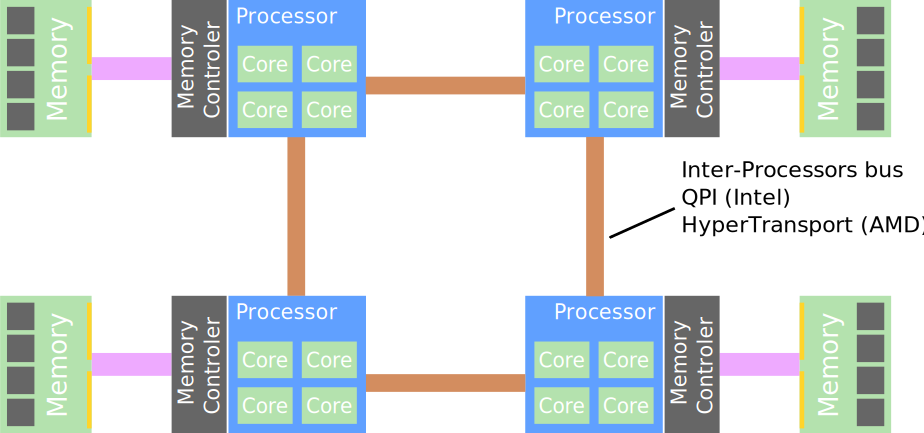
\includegraphics[width=0.8\textwidth]{numa}
  \caption{Vue d'ensemble d'une architecture NUMA.}
  \label{fig:numa}
\end{figure}
